
\documentclass[10pt]{article}

\def\Type{LessonDJ}
\def\TypeNum{Lesson 22}
\def\TypeTitle{Continuous Random Variables}
\def\Semester{Fall 2021} %Not Used 
\def\Course{MATH 1190 \& 1210}
\def\Targets{  {\bf\color{Orange}P2}, {\bf\color{Orange}P3} }

\usepackage{preambleDJ}

\usepackage{framed}


%%%%%%%%%%%% BEGIN DOCUMENT %%%%%%%%%%%%%%%
%%%%%%%%%%%% BEGIN DOCUMENT %%%%%%%%%%%%%%%
%%%%%%%%%%%% BEGIN DOCUMENT %%%%%%%%%%%%%%%
%%%%%%%%%%%% BEGIN DOCUMENT %%%%%%%%%%%%%%%
%%%%%%%%%%%% BEGIN DOCUMENT %%%%%%%%%%%%%%%




\begin{document}

\pagestyle{otherpages}
\thispagestyle{firstpage}
\vs{.65}


\blue{\bf Mini-Lecture: Continuous Random Variables \& Probability Density Functions}\\
Last lesson we introduced {\em Discrete Random Variables}. Today, we are talking about {\em Continuous Random Variables}. There are some similarities between these two and also some important differences.\\
\mpageT{.5}{.5}[\hs{.1}]{
\centering
\blue{ \bf Discrete Random Variables}
}{
\centering
\blue{ \bf Continuous Random Variables}
}\vs{-.2}
\itemNIN{
\mpageT{.5}{.5}[\hs{.2}]{
\item {\bf Discrete Example: } The random variable $X$ is the sum from randomly rolling two $4$-sided dice
}{
\item {\bf Continuous Example: } The random variable $T$ is the (random) wait time until the bus arrives  at the 
amphitheater on McIntyre. Buses arrive every $10$ minutes.
}
\vs{.0}\\
\mpageT{.5}{.5}[\hs{.2}]{
\item $S_X=\{2,3,4,5,6,7,8\}$
}{
\item $S_T=$%[a,b]=[0,10]$
}
\vs{.2}\\
\mpageT{.5}{.5}[\hs{.2}]{
\item {\bf Probability Mass Function}:  $f(k)$.\\
{ \em Two Properties:}
\enum{
\item $f(k)\geq0$ where $k\in S_X$
\item $\ds \sum_{k\in S_X}P[X=k] = \sum_{k=2}^8 P[X=k]=\sum_{k=2}^8 f(k)=1$
}
%
}{
\item {\bf Probability Density Function (PDF)}: $f(t)$.\\
{ \em Two Properties:}
\enum{
\item ~\\  %$f(t)\geq0$ where $t\in S_T$
\item %$\ds \int_a^b f(t)\;dt=\ds \int_0^{10} f(t)\;dt=1$ 
}
}

\mpageT{.5}{.5}[\hs{.2}]{
 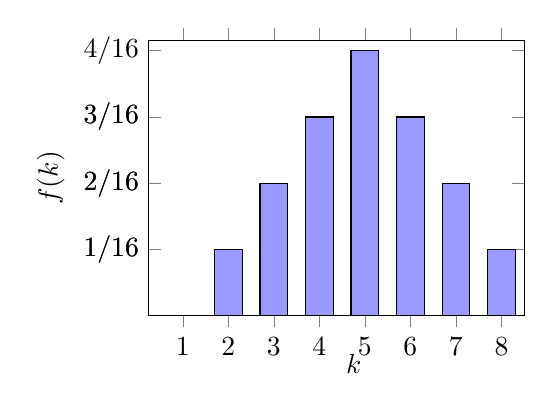
\begin{tikzpicture}
          \begin{axis}[
	ybar,
	bar shift = 0,
    	xtick=data,
            ytick       = {1/16, 2/16, 3/16,4/16,3/16,2/16,1/16},
            yticklabels =  {$1/16$, $2/16$, $3/16$,$4/16$,$3/16$,$2/16$,$1/16$},
            samples     = 160,
  		xmax=8.5,
            ymin = 0, ymax = .26,
            grid=none,
            width = 2.5in, height=2in,
            y label style={anchor=south},
            ylabel={$f(k)$},
                        xlabel = {$k$},
		x label style={anchor=west},
                 axis line style={->},
          ]
		\addplot[fill=blue!40] coordinates {(1,0)  (2,.0625)  (3,.125) (4,.1875) (5,.25) (6,.1875) (7,.125) (8,.0625) (9,0)};
        \end{axis}
        \end{tikzpicture}
}{
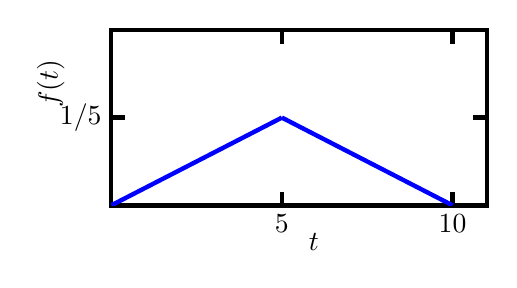
\begin{tikzpicture}
    \begin{axis}[
    	x label style={anchor=west},
            xlabel={$t$},
            xtick       = {5,10},
            xticklabels = {$5$,$10$},
            xticklabel style={anchor=north},
            y label style={anchor=west},
            ylabel={$f(t)$},
            ytick       = {1/5},
            yticklabels = {$1/5$},
            samples     = 320,
            domain      = -2.5:2.5,
            %restrict y to domain=-6.5:6.5,
            xmin =0, xmax = 11,
            ymin = 0, ymax = .4,
            axis line style = { ultra thick, ->},
            every major tick/.append style={ultra thick, black, major tick length=5pt},
            width=2.5in, height=1.5in
          %  grid=both, grid style=solid
          ]
    \addplot[domain=0:5, blue, ultra thick, mark=none]{1/25*x};
     \addplot[domain=5:10, blue, ultra thick, mark=none]{-1/25*x+2/5};
    \end{axis}
\end{tikzpicture}
}

}
\exercise\ltrm{\bf\color{Orange}P3}
Let's practice verifying that $f(x)$ is a {\bf PDF}.\\
Let $X$ be a continuous random variable with PDF given by:
\[
f(x) = 
\begin{cases} 
cx & \text{for } 0 \leq x \leq 2, \\
0 & \text{otherwise}.
\end{cases}
\]
\tasksA{2}{
\task  Find the support of $X$.\\


{\large
$S_X=$
}

\task  Find the value of the constant $c$ making $f$ a valid PDF.
}
\newpage


%%%%%%%%%
\newpage%
%%%%%%%%%
\blue{\bf Mini-Lecture: Cumulative Distribution Function (CDF)}\\
The Cumulative Distribution Function $F(x)$ is similar to the ``Area-so-far" function we encountered in our lesson the Fundamental Theorem of Calculus. A CDF represents the ``Probability-so-far." We again draw parallels between Discrete and Continuous Random Variables.\\
\mpageT{.5}{.5}[\hs{.2}]{
\centering {\bf  Discrete Random Variables}
}{
\centering {\bf Continuous Random Variables} 
}
\vs{-.2}
\itemNIN{
\mpageT{.5}{.5}[\hs{.2}]{
\item Our random variable $X$ is still  the sum from randomly rolling two $4$-sided dice.
}{
\item The random variable $T$ is still the (random) wait time until the bus arrives  at the 
amphitheater on McIntyre. Buses arrive every $10$ minutes. 
}%\\
\mpageT{.5}{.5}[\hs{.2}]{
 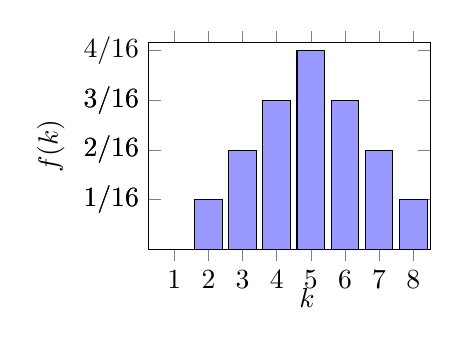
\begin{tikzpicture}
          \begin{axis}[
         scale=0.75,
	ybar,
	bar shift = 0,
    	xtick=data,
            ytick       = {1/16, 2/16, 3/16,4/16,3/16,2/16,1/16},
            yticklabels =  {$1/16$, $2/16$, $3/16$,$4/16$,$3/16$,$2/16$,$1/16$},
            samples     = 160,
  		xmax=8.5,
            ymin = 0, ymax = .26,
            grid=none,
            width = 2.5in, height=2in,
            y label style={anchor=south},
            ylabel={$f(k)$},
                        xlabel = {$k$},
		x label style={anchor=west},
                 axis line style={->},
          ]
		\addplot[fill=blue!40] coordinates {(1,0)  (2,.0625)  (3,.125) (4,.1875) (5,.25) (6,.1875) (7,.125) (8,.0625) (9,0)};
        \end{axis}
        \end{tikzpicture}
}{\hfill
 \begin{center}
 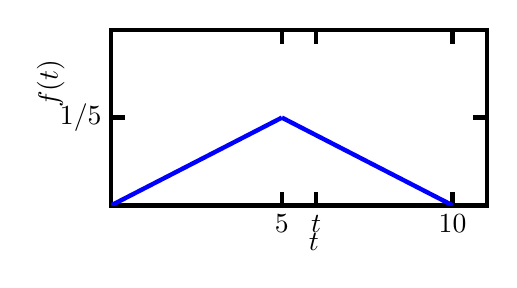
\begin{tikzpicture}
    \begin{axis}[
    scale=1,
    	x label style={anchor=west},
            xlabel={$t$},
            xtick       = {5,6,10},
            xticklabels = {$5$,$t$,$10$},
            xticklabel style={anchor=north},
            y label style={anchor=west},
            ylabel={$f(t)$},
            ytick       = {1/5},
            yticklabels = {$1/5$},
            samples     = 320,
            domain      = -2.5:2.5,
            %restrict y to domain=-6.5:6.5,
            xmin =0, xmax = 11,
            ymin = 0, ymax = .4,
            axis line style = { ultra thick, ->},
            every major tick/.append style={ultra thick, black, major tick length=5pt},
            width=2.5in, height=1.5in
          %  grid=both, grid style=solid
          ]
    \addplot[domain=0:5, blue, ultra thick, mark=none]{1/25*x};
     \addplot[domain=5:10, blue, ultra thick, mark=none]{-1/25*x+2/5};
    \end{axis}
\end{tikzpicture}
\end{center}
}
\mpageT{.5}{.5}[\hs{.2}]{
\item  {\bf  Cumulative Distribution  Function (CDF)} $$\ds F(k)=P[X\leq k]=\sum_{i=2}^k P[X=i]$$
}{
\item {\bf  Cumulative Distribution  Function (CDF)} $$\ds F(t)=P[T\leq t]=\int_a^t f(w)\;dw$$
}
}
\vs{1}
\mpageT{.5}{.5}[\hs{.2}]{
\example 
 What's the probability that someone will wait $3$ minutes or less to catch the bus? Find $F(3)$. {\em Hint} set up definite integral and use area of a common shape to compute it.
  \begin{center}
 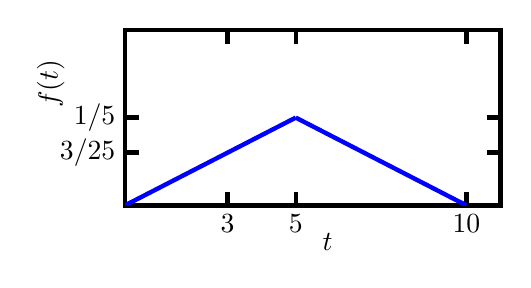
\begin{tikzpicture}
    \begin{axis}[
    scale=1,
    	x label style={anchor=west},
            xlabel={$t$},
            xtick       = {3,5,10},
            xticklabels = {$3$,$5$,$10$},
            xticklabel style={anchor=north},
            y label style={anchor=west},
            ylabel={$f(t)$},
            ytick       = {3/25, 1/5},
            yticklabels = {$3/25$,$1/5$},
            samples     = 320,
            domain      = -2.5:2.5,
            %restrict y to domain=-6.5:6.5,
            xmin =0, xmax = 11,
            ymin = 0, ymax = .4,
            axis line style = { ultra thick, ->},
            every major tick/.append style={ultra thick, black, major tick length=5pt},
            width=2.5in, height=1.5in
          %  grid=both, grid style=solid
          ]
       \addplot[domain=0:5, blue, ultra thick, mark=none]{1/25*x};
     \addplot[domain=5:10, blue, ultra thick, mark=none]{-1/25*x+2/5};
    \end{axis}
\end{tikzpicture}
\end{center}
}{
{\em Key Question} How do we find $\ds P[c\leq T\leq d]$?
 \begin{center}
 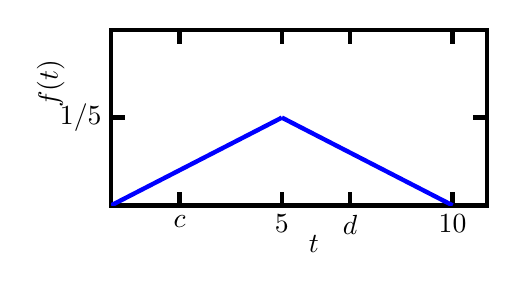
\begin{tikzpicture}
    \begin{axis}[
    scale=1,
    	x label style={anchor=west},
            xlabel={$t$},
            xtick       = {2,5,7,10},
            xticklabels = {$c$,$5$,$d$,$10$},
            xticklabel style={anchor=north},
            y label style={anchor=west},
            ylabel={$f(t)$},
            ytick       = {1/5},
            yticklabels = {$1/5$},
            samples     = 320,
            domain      = -2.5:2.5,
            %restrict y to domain=-6.5:6.5,
            xmin =0, xmax = 11,
            ymin = 0, ymax = .4,
            axis line style = { ultra thick, ->},
            every major tick/.append style={ultra thick, black, major tick length=5pt},
            width=2.5in, height=1.5in
          %  grid=both, grid style=solid
          ]
    \addplot[domain=0:5, blue, ultra thick, mark=none]{1/25*x};
     \addplot[domain=5:10, blue, ultra thick, mark=none]{-1/25*x+2/5};
    \end{axis}
\end{tikzpicture}
\end{center}
% \al{
% P[c\leq T\leq d]&=P[T\leq d]-P[T\leq c]\\
% &=\int_0^df(t)\;dt-\int_0^cf(t)\;dt\\
% P[c\leq T\leq d] &=\int_c^d f(t)\;dt
% }
}


\newpage
\exercise\ltrm{\bf\color{Orange}P3} Let's return to the PDF from Exercise A.  $X$ is a continuous random variable with PDF given by:
\[
f(x) = 
\begin{cases} 
cx & \text{for } 0 \leq x \leq 2, \\
0 & \text{otherwise}.
\end{cases}
\]


\tasksA{2}{

\task Use the value of $c$ you found in Exercise A and  find the probability that $X$ takes on a value less than or equal to $1.5$. That is find \\$P[X\leq 1.5]=F(1.5)$
\task What's $P[X=1.5]$?  Think about how to set up a definite integral that might represent this quantity.  \vs{2.5}





\task Give an example of an interval $[c,d]$ that $X$ has a $25\%$ chance of falling in (there are many reasonable answers!). Show your answer is correct.



}

\newpage
\exercise\ltrm{\bf\color{Orange}P3}
The PDF of the continuous random variable $X$ is given below:\\

\

\,\hfill
%
\begin{minipage}[t][0.5in]{0.25\textwidth}
$
f(x) = 
\begin{cases} 
1 & \text{for } 0 \leq x \leq 1, \\
0 & \text{otherwise},
\end{cases}
$
\end{minipage}
%
\hfill
%
\begin{minipage}[t][0.5in]{0.25\textwidth}
\,\\[-0.5in]
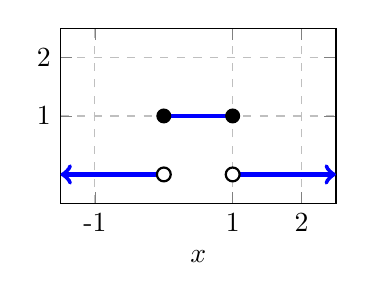
\begin{tikzpicture}
          \begin{axis}[
        %    axis y line = left,
        %    axis x line = bottom,
            xlabel = {$x$},
            xtick       = {-1,1,2},
            xticklabels = {-1,1,2},
            ytick       = {1,2},
            yticklabels = {1,2},
            samples     = 160,
            domain      = -1:3,
            restrict y to domain=-0.1:4,
            xmin = -1.5, xmax = 2.5,
            ymin = -0.5, ymax = 2.5,
            width = 2in, height=1.5in,
            grid=both, grid style=dashed
          ]
          \draw[ultra thick,blue,<-] (-1.5,0) -- (0,0);
          \draw[ultra thick,blue] (0,1) -- (1,1);
          \draw[ultra thick,blue,->] (1,0) -- (2.5,0);
          \filldraw (0,1) circle (2.5pt);
          \filldraw (1,1) circle (2.5pt);
          \filldraw[fill=white, thick] (1,0) circle (2.5pt);
          \filldraw[fill=white, thick] (0,0) circle (2.5pt);
        \end{axis}
\end{tikzpicture}
\end{minipage}
%
\hfill\,\\

\begin{itemize}
\item[(a)] Use the formula in the mini-lecture to find $F(x)$, the CDF of $X$.



\end{itemize}
\vs{2}
\begin{minipage}[t]{0.5\textwidth}
\begin{itemize}
\item[(b)] Sketch the graph of the CDF $F(x)$.

    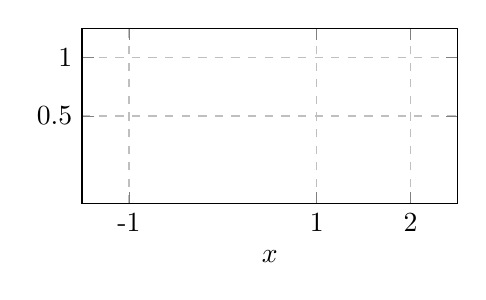
\begin{tikzpicture}
          \begin{axis}[
        %    axis y line = left,
        %    axis x line = bottom,
            xlabel = {$x$},
            xtick       = {-1,1,2},
            xticklabels = {-1,1,2},
            ytick       = {1,2},
            yticklabels = {0.5,1},
            samples     = 160,
            domain      = -1:3,
            restrict y to domain=-0.1:4,
            xmin = -1.5, xmax = 2.5,
            ymin = -0.5, ymax = 2.5,
            width = 2.5in, height=1.5in,
            grid=both, grid style=dashed
          ]
        \end{axis}
    \end{tikzpicture}
\end{itemize}
\end{minipage}
%
\begin{minipage}[t]{0.45\textwidth}
    \begin{itemize}
    \item[(c)] Find the number $m$ for which $P(X<m)=0.5$. ({\bf Note:} this number $m$ is called the {\bf median} of $X$.)
    \end{itemize}
\end{minipage}\\

\

%%%%%%%%%
\newpage%
%%%%%%%%%
{\exercise}\ltrm{\bf\color{Orange}P3}
Consider the PDF of the random variable $Z$:
\[
f(z) = 
\begin{cases} 
\dfrac{1}{12}z & \text{for } 1 \leq z \leq 5, \\
0 & \text{otherwise}.
\end{cases}
\]
\tasksA{2}{

\task Find $P(2\leq Z\leq 4)$.

    
\task Find $F(z)$, the CDF of $Z$\vs{3}
\task \blue{\bf(Extra Practice)} Find the median of $Z$.

}

\newpage

{\bf\color{blue}Extra Practice 1.} \ltrm{\bf\color{Orange}P3}Consider the PDF:
\[
    f(x) = 
    \begin{cases} 
    cx(1 - x) & \text{for } 0 \leq x \leq 1, \\
    0 & \text{otherwise}.
    \end{cases}
\]
\begin{enumerate}
\item[(a)] Find the value of $c$ making $f$ a valid PDF.
    
\vfill

\item[(b)] Suppose you know $X$ has a 75\% chance to fall in the interval $[a,1]$. Find $a$.

\vfill

\item[(c)] Suppose you know $X$ has a 25\% chance to fall in the interval $[0,b]$. Find $b$.

\vfill

\item[(d)] What do you notice about $a$ and $b$? How is this relationship related to the fact that $\displaystyle\int_0^1 f(x)\,dx$ must equal $1$? ({\bf Hint:} you might want to use a property of definite integrals to explain your answer.)

\vfill

\end{enumerate}

%%%%%%%%%
\newpage%
%%%%%%%%%

{\bf\color{blue}Extra Practice 2.} \ltrm{{\bf\color{Orange}P3}}
For the PDF given by:
\[
f(x) = 
\begin{cases} 
3x^2 & \text{for } 0 \leq x \leq 1, \\
0 & \text{otherwise},
\end{cases}
\]
Find and graph the CDF $F(x)$.\\

\vs{3}
\,\hfill
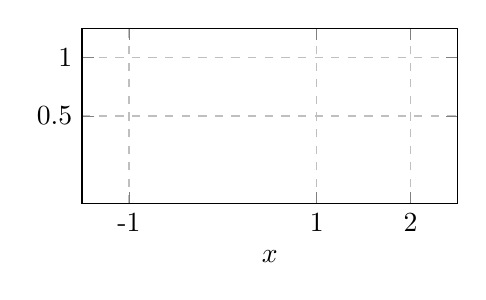
\begin{tikzpicture}
          \begin{axis}[
        %    axis y line = left,
        %    axis x line = bottom,
            xlabel = {$x$},
            xtick       = {-1,1,2},
            xticklabels = {-1,1,2},
            ytick       = {1,2},
            yticklabels = {0.5,1},
            samples     = 160,
            domain      = -1:3,
            restrict y to domain=-0.1:4,
            xmin = -1.5, xmax = 2.5,
            ymin = -0.5, ymax = 2.5,
            width = 2.5in, height=1.5in,
            grid=both, grid style=dashed
          ]
        \end{axis}
    \end{tikzpicture}

\



\end{document}